% -----------------------------------------------------------
\section{การออกแบบระบบการเล่น}
% -----------------------------------------------------------

\subsection{วิธีการเล่นเกม (How to Play)}

ในการเล่นเกมนี้ ผู้เล่นจะได้รับบทเป็นกัปตันเรือขนส่งสินค้า โดยมีหน้าที่ในการสั่งการลูกเรือเพื่อนำพาเรือเดินทางไปยังจุดหมายปลายทางอย่างปลอดภัย โดยกติกาการเล่นหลักมีดังนี้

\begin{enumerate}[label=\arabic*)]
    \item \textbf{เริ่มต้นภารกิจ:} ผู้เล่นเริ่มเกมด้วยการรับทราบเส้นทางเดินเรือและสภาพแวดล้อมเบื้องต้น
    \item \textbf{การควบคุมผ่านเสียง:} ผู้เล่นไม่สามารถใช้คีย์บอร์ดหรือเมาส์บังคับพวงมาลัยเรือโดยตรง แต่ต้องใช้ \textbf{คำสั่งเสียงภาษาอังกฤษ} (Voice Commands) สื่อสารกับลูกเรือ AI (พลต้นหน และ พลถือท้าย)
    \item \textbf{การหลบหลีกสิ่งกีดขวาง:} เมื่อเกมสุ่มสร้างสิ่งกีดขวาง (Obstacles) เช่น โขดหิน เกาะ หรือเรือลำอื่น ผู้เล่นต้องวิเคราะห์สถานการณ์จากมุมมองไอโซเมตริกและหน้าจอเรดาร์ จากนั้นออกคำสั่งที่เหมาะสม (เช่น "Starboard 15", "Stop Engine") ให้ทันเวลา
    \item \textbf{การตอบสนองของลูกเรือ:} 
    \begin{itemize}
        \item หากคำสั่งถูกต้องและชัดเจน พลถือท้ายจะบังคับเรือตามหลักฟิสิกส์ (มีแรงเฉื่อยและรัศมีวงเลี้ยว)
        \item หากคำสั่งไม่ถูกต้อง ผิดบริบท หรือออกเสียงไม่ชัดเจน ลูกเรือ AI จะทวนคำสั่งหรือขอให้ย้ำคำสั่ง (Clarification Request) ทำให้ผู้เล่นต้องเปล่งเสียงใหม่
    \end{itemize}
    \item \textbf{ผลลัพธ์ของภารกิจ:} 
    \begin{itemize}
        \item \textbf{สำเร็จ (Victory):} หากนำเรือถึงจุดหมายโดยหลบหลีกสิ่งกีดขวางได้ทั้งหมด
        \item \textbf{ล้มเหลว (Game Over):} หากชนสิ่งกีดขวางจนมาตรวัดความเสียหาย (Hull Integrity) ลดลงเหลือศูนย์
    \end{itemize}
\end{enumerate}

\subsection{กระบวนการเล่นหลัก (Core Game Loop)}

กระบวนการทำงานหลักของการเล่นเกม (Core Game Loop) ซึ่งสะท้อนการโต้ตอบระหว่างผู้เล่น, AI, และระบบฟิสิกส์ แสดงดังภาพที่ \ref{fig:gameloop}

\begin{figure}[H]
\centering
\begin{mermaid}
graph TD
    A[เริ่มภารกิจ] --> B[ประเมินสถานการณ์จากเรดาร์/สภาพแวดล้อม]
    B --> C{พบสิ่งกีดขวางหรือไม่?}
    C -- ไม่พบ --> D[รักษาเส้นทางและระดับความเร็ว]
    D --> B
    C -- พบสิ่งกีดขวาง --> E[ผู้เล่นออกคำสั่งเสียงภาษาอังกฤษฉุกเฉิน]
    E --> F[ระบบแปลงเสียงเป็นข้อความ Speech-to-Text]
    F --> G{คำสั่งชัดเจนและถูกต้องหรือไม่?}
    G -- ไม่ถูกต้อง/ไม่ชัดเจน --> H[ลูกเรือ AI จำลองการสื่อสารติดขัด และขอให้ย้ำคำสั่ง]
    H --> E
    G -- ถูกต้อง --> I[ลูกเรือ AI รับคำสั่งและตอบกลับ]
    I --> J[ระบบฟิสิกส์ควบคุมเรือเคลื่อนที่ตามคำสั่ง]
    J --> K{หลบหลีกสำเร็จหรือไม่?}
    K -- สำเร็จ --> L{ถึงจุดหมายหรือยัง?}
    L -- ยังไม่ถึง --> B
    L -- ถึงแล้ว --> M[ภารกิจสำเร็จ Victory]
    K -- ไม่สำเร็จ ชนสิ่งกีดขวาง --> N[มาตรวัดความเสียหาย Hull Integrity ลดลง]
    N --> O{ความเสียหายเหลือ 0 หรือไม่?}
    O -- ยังไม่เหลือ 0 --> B
    O -- เหลือ 0 --> P[ภารกิจล้มเหลว Game Over]
\end{mermaid}
\caption{แผนภาพกระบวนการเล่นหลัก (Core Game Loop)}
\label{fig:gameloop}
\end{figure}

จากภาพที่ \ref{fig:gameloop} แสดงให้เห็นว่าความท้าทายหลักของเกมไม่ได้อยู่ที่การบังคับปุ่ม แต่เป็นการบริหารเวลาในการ "เปล่งเสียง" และ "แก้ปัญหาการสื่อสาร" ภายใต้สถานการณ์ที่ระบบฟิสิกส์ของเรือยังคงดำเนินไปอย่างต่อเนื่อง

\subsection{การออกแบบส่วนติดต่อผู้ใช้ (UI/HUD Design)}

การออกแบบหน้าจอส่วนติดต่อผู้ใช้ (UI/HUD) ถูกออกแบบภายใต้แนวคิดการจำลองสถานการณ์ (Simulation Game Design) เพื่อให้ข้อมูลที่จำเป็นครบถ้วนแต่ไม่บดบังทัศนวิสัยหลัก รายละเอียดของส่วนประกอบบนหน้าจอ แสดงดังตารางที่ \ref{tab:hud}

\begin{table}[H]
\centering
\caption{องค์ประกอบของหน้าจอส่วนติดต่อผู้ใช้ (HUD)}
\label{tab:hud}
\begin{tabular}{|p{4.5cm}|p{9.2cm}|}
\hline
\textbf{องค์ประกอบหน้าจอ} & \textbf{บทบาทและหน้าที่} \\
\hline
มาตรวัดการเดินเรือ (Navigation Instruments) & แสดงเข็มทิศบอกองศาทิศทาง (Compass) และตัวแสดงองศาของพวงมาลัยหางเสือ (Rudder Angle Indicator) เพื่อให้กัปตันประเมินทิศทาง \\ \hline
สถานะเครื่องยนต์ (Engine Telegraph) & แสดงระดับความเร็วของเรือในปัจจุบัน \\ \hline
หน้าจอเรดาร์ (Radar Screen) & แสดงจุดของสิ่งกีดขวาง (Blips) รอบตัวเรือ เพื่อช่วยประเมินสถานการณ์ล่วงหน้า \\ \hline
สถานะการรับเสียง (Voice Input Indicator) & สัญลักษณ์รูปไมโครโฟนเพื่อแจ้งผู้เล่นว่าขณะนี้ระบบกำลังรับฟังเสียง หรือกำลังประมวลผลคำสั่ง \\ \hline
มาตรวัดความเสียหาย (Hull Integrity) & แถบพลังชีวิต (Health Bar) ของเรือ หากเกิดการชนแถบนี้จะลดลง \\
\hline
\end{tabular}
\end{table}

\pagebreak
\subsection{สถาปัตยกรรมของระบบ (System Architecture)}

สถาปัตยกรรมระบบเกมเดินเรือด้วยระบบสั่งการด้วยเสียงแสดงดังภาพที่ \ref{fig:architecture}

\begin{figure}[H]
\centering
\begin{mermaid}
graph TD
    subgraph Client["ส่วนของผู้เล่น (Client)"]
        Unity["Unity 3D Engine (Game Client)"]
        Mic["Microphone (Audio Input)"]
        Speaker["Speaker/Headphones (Audio Output)"]
    end

    subgraph Core["ส่วนประมวลผลหลัก (Core Systems)"]
        GameLogic["C# Game Logic & Ship Physics"]
        UI["UI & HUD Manager"]
    end

    subgraph ExternalAPI["ส่วนเชื่อมต่อภายนอก (External APIs)"]
        STT["Speech-to-Text API (Whisper)"]
        LLM["OpenAI API (GPT-4o mini)"]
    end

    Mic -->|Voice Input| Unity
    Unity -->|Audio Stream| STT
    STT -->|Text| GameLogic
    GameLogic -->|Text Prompt| LLM
    LLM -->|Voice/Text Feedback| GameLogic
    GameLogic -->|Control| UI
    GameLogic -->|Audio Feedback| Speaker
\end{mermaid}
\caption{สถาปัตยกรรมของระบบเกม}
\label{fig:architecture}
\end{figure}

จากภาพที่ \ref{fig:architecture} ระบบทำงานบน Game Engine Unity 3D เป็นหลัก โดยรับเสียงพูดภาษาอังกฤษผ่านไมโครโฟน ส่งไปแปลงเป็นข้อความด้วยเทคโนโลยีการรู้จำเสียง (Whisper API)\cite{aguirre2023} จากนั้นนำข้อความไปประมวลผลคำสั่งร่วมกับระบบฟิสิกส์เรือ หรือส่งต่อให้ปัญญาประดิษฐ์ (OpenAI GPT-4o mini) เพื่อสร้างบทสนทนาโต้ตอบจากลูกเรือ AI

\subsection{โครงสร้างโฟลเดอร์ของโครงการ (Project Structure)}

โครงสร้างแฟ้มข้อมูลของการพัฒนาโครงการบน Unity 3D แสดงดังตารางที่ \ref{tab:folder}

\begin{table}[H]
\centering
\caption{โครงสร้างโฟลเดอร์หลักของโครงการ}
\label{tab:folder}
\begin{tabular}{|p{4.5cm}|p{9.2cm}|}
\hline
\textbf{โฟลเดอร์} & \textbf{คำอธิบาย} \\
\hline
\texttt{Assets/Scenes/} & ฉากต่าง ๆ ภายในเกม (MainMenu, Gameplay, Shipyard, Result) \\ \hline
\texttt{Assets/Scripts/} & ชุดคำสั่งภาษา C\# สำหรับควบคุมระบบฟิสิกส์เรือ การรับคำสั่งเสียง และระบบ UI \\ \hline
\texttt{Assets/Scripts/API/} & ชุดคำสั่งสำหรับเชื่อมต่อ Speech-to-Text (Whisper) และ OpenAI API \\ \hline
\texttt{Assets/Prefabs/} & วัตถุสำเร็จรูป เช่น ตัวเรือ สิ่งกีดขวางที่ใช้ในการสุ่ม (Obstacle Generation) \\ \hline
\texttt{Assets/Models/} & แฟ้มโมเดล 3 มิติ (3D Models) ของเรือ สิ่งแวดล้อม และสิ่งกีดขวาง \\ \hline
\texttt{Assets/Audio/} & แฟ้มเสียงสภาพแวดล้อม (Ambient Audio) และเสียงเอฟเฟกต์ (SFX) สัญญาณเตือน \\ \hline
\texttt{Assets/UI/} & รูปภาพและกราฟิกสำหรับหน้าจอเรดาร์ เข็มทิศ และอินเทอร์เฟซผู้ใช้ \\
\hline
\end{tabular}
\end{table}

\subsection{การออกแบบหน้าจอ (UI Mockups)}

ต้นแบบหน้าจอ (Mockups) สำหรับเกมถูกออกแบบเพื่อจำลองสถานการณ์การเดินเรือ (Simulation) ให้ดูสมจริงและอ่านข้อมูลง่าย โดยมีหน้าจอหลักดังตารางที่ \ref{tab:mockups}

\begin{table}[H]
\centering
\caption{รายการต้นแบบหน้าจอ}
\label{tab:mockups}
\begin{tabular}{|p{1.5cm}|p{3.5cm}|p{8.5cm}|}
\hline
\textbf{รหัสหน้าจอ} & \textbf{ชื่อหน้าจอ} & \textbf{ส่วนประกอบหลัก} \\
\hline
UI-01 & หน้าจอหลัก (Main Menu) & ชื่อเกม, ปุ่มเริ่มเกม (Start Game), ปุ่มตั้งค่าระบบเสียง, ปุ่มออกเกม (Exit) \\ \hline
UI-02 & หน้าจอเล่นเกม (Gameplay HUD) & มุมมองไอโซเมตริกของเรือ, เข็มทิศ, หน้าจอเรดาร์, สถานะความเร็ว, สถานะไมโครโฟน, แถบความเสียหายเรือ \\ \hline
UI-03 & หน้าจออู่ต่อเรือ (Shipyard) & เมนูศูนย์กลางสำหรับนำเงินรางวัลมาซ่อมแซมหรืออัปเกรดประสิทธิภาพเรือ \\ \hline
UI-04 & หน้าจอสรุปผล (Result Screen) & หน้าจอแสดงผลเมื่อถึงเป้าหมายหรือเมื่อเรืออับปาง สรุปคะแนนความแม่นยำในการออกเสียง ความรวดเร็วในการสั่งการ \\
\hline
\end{tabular}
\end{table}

\subsubsection{UI-02: หน้าจอเล่นเกม (Gameplay HUD)}

หน้าจอส่วนติดต่อผู้ใช้ขณะเล่นเกมเป็นหน้าจอหลักที่ผู้เล่นจะต้องใช้งานตลอดการทำภารกิจ ออกแบบตามมุมมองไอโซเมตริก (Isometric View) แสดงภาพจำลองการจัดวางดังภาพที่ \ref{fig:wf_gameplay}

\begin{figure}[H]
\centering
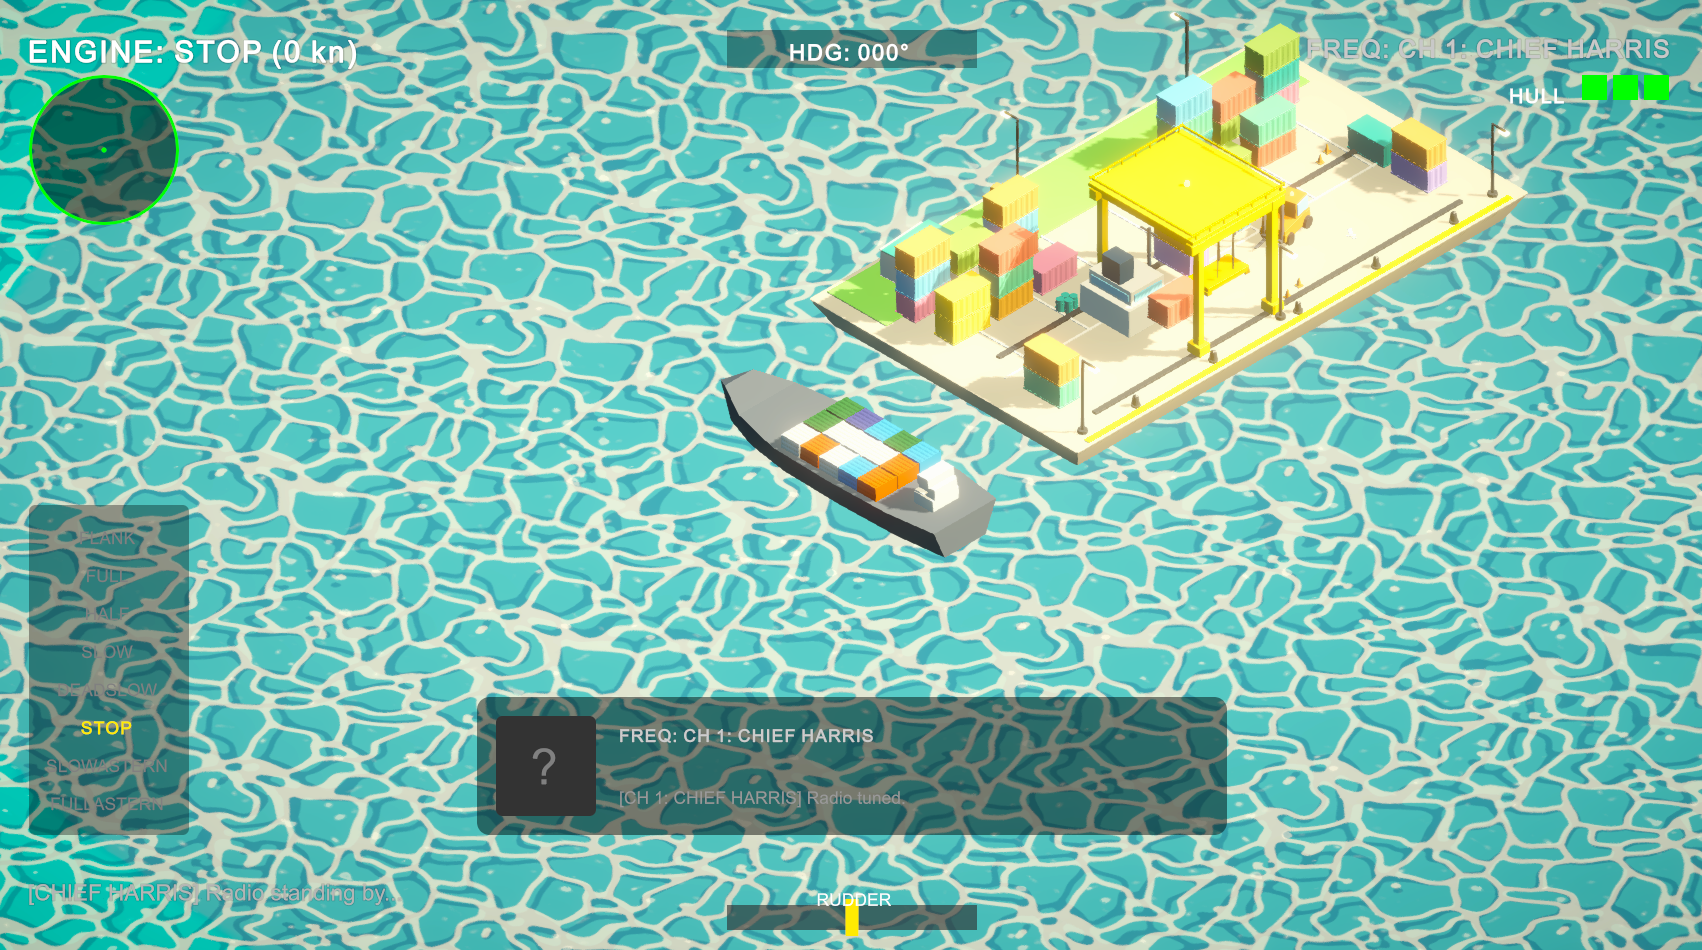
\includegraphics[width=0.8\textwidth]{Document/GameDev/images/StartUI.png}
\caption{ต้นแบบหน้าจอเล่นเกม (UI-02)}
\label{fig:wf_gameplay}
\end{figure}

จากภาพที่ \ref{fig:wf_gameplay} ผู้เล่นจะมองเห็นเรือจากมุมมองไอโซเมตริก เพื่อให้เห็นตัวเรือ สภาพแวดล้อมทางทะเล และตำแหน่งของสิ่งกีดขวางโดยรอบได้อย่างชัดเจน มุมหน้าจอจะมีมาตรวัดการเดินเรือ ได้แก่ เรดาร์ เข็มทิศบอกองศาทิศทาง และมาตรวัดความเร็ว นอกจากนี้ ด้านล่างจะมีสัญลักษณ์ไมโครโฟน (Voice Input Indicator) เพื่อแสดงสถานะว่าระบบกำลังรับฟัง หรือกำลังประมวลผลคำสั่ง เพื่อให้ผู้เล่นสามารถจับจังหวะการพูดและบริหารเวลาในการสื่อสารได้อย่างถูกต้อง